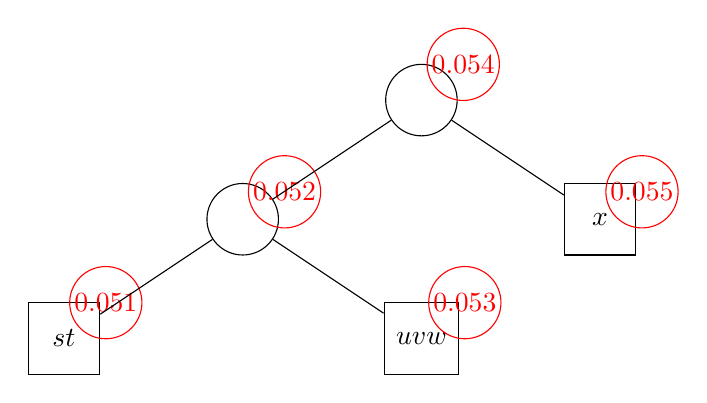
\begin{tikzpicture}
  [state/.style={circle,draw,minimum size=12ex,inner sep=0.075cm}
  ,leaf/.style={rectangle,draw,minimum size=12ex,inner sep=1ex}
  ,nr/.style={circle,red,draw,yshift=3ex,xshift=2pt,inner sep=1pt}
  , scale=1
  , thin]

  \draw (00ex,  00ex) node[state,minimum size=6ex]  (s0) {\(\alt\)};
  \draw (-15ex, -10ex) node[state,minimum size=6ex] (s1) {\(\alt\)};
  \draw (-30ex, -20ex) node[leaf,minimum size=6ex]  (s2) {\(s \seq t\)};
  \draw ( 00ex, -20ex) node[leaf,minimum size=6ex]  (s3) {\(u \seq v \seq w\)};
  \draw ( 15ex, -10ex) node[leaf,minimum size=6ex]  (s4) {\(x\)};

  \draw (s2.east) node[nr]  () {\(\scalefont{0.05} 1\)};
  \draw (s1.east) node[nr,yshift=-3pt]  () {\(\scalefont{0.05} 2\)};
  \draw (s3.east) node[nr]  () {\(\scalefont{0.05} 3\)};
  \draw (s0.east) node[nr]  () {\(\scalefont{0.05} 4\)};
  \draw (s4.east) node[nr,yshift=-3pt]  () {\(\scalefont{0.05} 5\)};

  % Paths
  \path (s0) edge[] node[align=left,above] {} (s1);
  \path (s1) edge[] node[align=left,above] {} (s2);
  \path (s1) edge[] node[align=left,above] {} (s3);
  \path (s0) edge[] node[align=left,above] {} (s4);

\end{tikzpicture}


%%% Local Variables:
%%% mode: latex
%%% TeX-master: "paper"
%%% End:
